% Sección 7: Integración de la solución, aplicación web y visualización
% evidencia:E20,E21,E22,E23,E28

\section{Integración de la solución, aplicación web y visualización}

La arquitectura de MediFlow desacopla la extracción agregada sobre la base hospitalaria respecto de la capa de servicio HTTP, la aplicación interactiva de usuario y el tablero histórico de inteligencia de negocios. Esta separación impide que la interfaz web o el usuario final accedan a la base PostgreSQL o a archivos Parquet con series hospitalarias cuando el sistema opera en modo de producción \parencite{mediflow2026informe}.

\subsection{Arquitectura modular y contratos HTTP de la API}

La Figura~\ref{fig:arquitectura_tikz} esquematiza conceptualmente las capas implementadas en el repositorio. A partir de la base PostgreSQL de solo lectura, las consultas SQL \texttt{00}--\texttt{23} generan agregados en \texttt{data/raw/}, que alimentan dos ramas paralelas: hacia la izquierda de la solución operativa, el paquete Python \texttt{hun} (junto con los insumos calendáricos de \texttt{src/external/}) entrena los modelos y serializa el artefacto \texttt{models/modelos\_web\_bundle.joblib} consumido por FastAPI y React/Vite; hacia la rama de análisis histórico, el script \texttt{preparar\_modelo.py} genera el modelo estrella consumido por Power BI Desktop bajo formato PBIP \parencite{mediflow2026informe,mediflow2026pbip}.

\begin{figure}[htbp]
\caption{Esquema conceptual de la arquitectura de implementación de MediFlow}
\label{fig:arquitectura_tikz}
\centering
{\singlespacing\footnotesize
\resizebox{\textwidth}{!}{%
\begin{tikzpicture}[
  node distance=7mm and 7mm,
  box/.style={draw=black!75, rounded corners=2pt, align=center, inner sep=5pt, minimum height=9mm, font=\footnotesize},
  priv/.style={box, fill=black!5},
  prod/.style={box, fill=black!10, thick},
  ext/.style={box, dashed},
  arr/.style={-{Stealth[length=2.2mm]}, semithick}
]
  \node[priv] (pg) {PostgreSQL HUN\\(OMOP solo lectura, VPN)};
  \node[priv, right=of pg] (sql) {SQL \texttt{00}--\texttt{23}\\Agregados \texttt{data/raw/}};
  \node[ext, below=of sql] (extd) {\texttt{src/external/}\\Calendario, clima, SIVIGILA};
  \node[priv, right=of sql] (hun) {Paquete \texttt{hun}\\Entrenamiento y empaquetado};
  \node[prod, right=of hun] (bundle) {Bundle \texttt{v2.0}\\(\texttt{.joblib}, corte \texttt{2026-07-17})};
  \node[prod, below=of bundle] (api) {API FastAPI\\15 rutas HTTP\\(\texttt{HUN\_MODO\_PRODUCCION=1})};
  \node[prod, left=of api] (web) {Frontend React / Vite\\5 vistas + simulador};
  \node[ext, below=of api] (chat) {\texttt{POST /api/chat}\\6 herramientas + respaldo};
  \node[priv, above=of sql] (pbi_prep) {\texttt{preparar\_modelo.py}\\(corte \texttt{2026-04-30})};
  \node[box, right=of pbi_prep] (pbip) {Proyecto PBIP Power BI\\7 pág., 12 tab., 43 medidas};

  \draw[arr] (pg) -- (sql);
  \draw[arr] (sql) -- (hun);
  \draw[arr] (extd) -- (hun);
  \draw[arr] (hun) -- node[above, font=\scriptsize]{\tiny offline} (bundle);
  \draw[arr] (bundle) -- (api);
  \draw[arr] (api) -- (web);
  \draw[arr] (api) -- (chat);
  \draw[arr] (sql) -- (pbi_prep);
  \draw[arr] (pbi_prep) -- (pbip);
\end{tikzpicture}%
}
}
\apanota{Esquema conceptual elaborado a partir de \texttt{app/api/\_\_init\_\_.py}, \texttt{src/hun/models/empaquetar.py} y \texttt{dashboards/powerbi/}. Representa exclusivamente componentes implementados en el repositorio sin añadir integraciones HIS en tiempo real ni sistemas clínicos externos inexistentes. El bloque \texttt{src/external/} genera insumos para entrenamiento; en producción estricta, FastAPI lee únicamente el bundle autorizado sin consultar \texttt{data/}.}
\end{figure}

La inspección directa de \texttt{app/api/\_\_init\_\_.py} y \texttt{app/api/chat.py} confirma \textbf{15 rutas HTTP reales} vigentes (cuyo inventario completo figura en el Anexo~C): \texttt{GET /api/health} (no existe \texttt{/api/salud}), \texttt{GET /api/modelo}, \texttt{GET /api/servicios}, \texttt{GET /api/parametros}, \texttt{GET /api/turnos/\{servicio\}}, \texttt{GET /api/ocupacion}, \texttt{GET /api/cuellos-botella}, \texttt{GET /api/comparacion/\{servicio\}}, \texttt{GET /api/efectos-eventos/\{servicio\}}, \texttt{GET /api/largo-plazo/\{servicio\}}, \texttt{GET /api/optimizacion}, \texttt{POST /api/predecir}, \texttt{POST /api/predecir-rango}, \texttt{POST /api/optimizacion/simular} y \texttt{POST /api/chat}. Las menciones históricas a \texttt{/api/historico/llegadas}, \texttt{/api/historico/turnos} o \texttt{/api/salud} en documentos anteriores (\texttt{DEC-007} y \texttt{tests/README.md}) están superadas por la implementación actual.

Tres salvaguardas técnicas delimitan el alcance de la API \parencite{mediflow2026auditoria}:
\begin{enumerate}[leftmargin=*,nosep]
\item \textit{Modo estricto sin datos crudos}: cuando \texttt{HUN\_MODO\_PRODUCCION=1} (o \texttt{HUN\_ENV=production}), \texttt{predict.py} carga únicamente \texttt{models/modelos\_web\_bundle.joblib} (o \texttt{HUN\_BUNDLE\_PATH}). Si el artefacto falta o falla la inferencia, la API devuelve código HTTP \texttt{503} sin acudir a archivos Parquet ni degradar silenciosamente a parámetros fijos.
\item \textit{Separación entre aceptación HTTP y validación científica}: \texttt{RangoRequest} admite horizontes de 1 a 30 días, pero esa aceptación sintáctica no demuestra validación predictiva a 30 días (los backtests operativos cubren 1--7 días). De igual modo, \texttt{GET /api/ocupacion} devuelve indicadores calculados sobre llegadas diarias relativas a $p_{75}/p_{90}$ históricos, no ocupación física sobre camas instaladas.
\item \textit{CORS y dependencia del backend}: la variable \texttt{ALLOWED\_ORIGINS} restringe los orígenes de navegador en CORS, pero no sustituye un mecanismo de autenticación o control de acceso de usuarios. La aplicación web React/Vite requiere la API FastAPI activa y no opera de forma autónoma sin backend.
\end{enumerate}

\subsection{Asistente conversacional de solo lectura (\texttt{/api/chat})}

El módulo \texttt{app/api/chat.py} implementa un asistente restringido exclusivamente a \textbf{seis herramientas deterministas de solo lectura} sobre las salidas del modelo y el estado visible en pantalla: \texttt{predecir}, \texttt{predecir\_rango}, \texttt{simular\_escenario}, \texttt{efecto\_promedio\_evento}, \texttt{indicadores\_cuellos\_botella} y \texttt{recomendaciones\_optimizacion}. El asistente carece de acceso SQL, no consulta filas de pacientes y no puede emitir órdenes médicas. Incorpora filtro para consultas fuera de tema, límite de 20 solicitudes por minuto por cliente, tiempo máximo de espera de 12\,s y recorte a 150 palabras. En el código figura configurado el identificador de modelo \texttt{claude-haiku-5-5} mediante la variable de entorno \texttt{ANTHROPIC\_API\_KEY}; ante ausencia de clave o falla de proveedor externo, el endpoint conmuta a un respaldo determinista offline sobre las mismas herramientas agregadas \parencite{mediflow2026informe}. Este respaldo local no convierte a la aplicación web completa en una plataforma autónoma sin servidor FastAPI.

\subsection{Tablero histórico en Power BI (PBIP) y estado de publicación}

La definición local versionada en \texttt{dashboards/powerbi/HUN\_CuellosBotella/} fue inspeccionada directamente sobre \texttt{model.bim} y las definiciones de páginas y visuales \parencite{mediflow2026pbip}. El modelo estrella está integrado por \textbf{12 tablas} (5 dimensiones, 6 tablas de hechos y la tabla \texttt{\_Medidas}), \textbf{18 relaciones}, \textbf{43 medidas DAX} y \textbf{7 páginas} (Inicio, Resumen ejecutivo, Saturación por área, Esperas y flujo, Demanda, Hallazgos y recomendaciones, Metodología y glosario), con parámetro de corte fijado en \texttt{FechaCorte = 2026-04-30}.

Es necesario documentar dos precisiones críticas sobre el tablero. Primera, durante el cierre de auditoría se corrigieron textos locales en visuales del PBIP (por ejemplo, \texttt{esperasv12}, \texttt{hallazgosv02}, \texttt{hallazgosv03}, \texttt{metodologiav02} y \texttt{metodologiav03}) para eliminar la equiparación entre marcas OMOP y espera por cama o promesas causales sobre el $p_{90}$; sin embargo, el archivo PBIP no contiene datos y el enlace público de Power BI no se ha vuelto a verificar ni se ha republicado tras dichas ediciones locales \parencite{mediflow2026auditoria}. Segunda, persiste una discrepancia documental no reconciliada sobre las fechas: \texttt{dashboards/README.md} justifica el corte de abril señalando que desde mayo de 2026 la extracción viene incompleta, mientras \texttt{docs/inventario\_base.md} reporta ausencia de meses vacíos hasta junio de 2026 y último día completo el 16 de julio de 2026. Ambas cohortes deben mantenerse diferenciadas en toda interpretación ejecutiva.

\subsection{Lectura crítica de las capturas archivadas de la interfaz}

Las Figuras~\ref{fig:app_cuellos} a \ref{fig:app_dashboard} documentan la interfaz web construida en React, Vite y Tailwind CSS como \textbf{evidencia visual archivada} previa al cierre documental \parencite{mediflow2026informe}. Su examen técnico exige las siguientes aclaraciones de trazabilidad:

\begin{itemize}[leftmargin=*,nosep]
\item \textit{Cuellos de botella} (Figura~\ref{fig:app_cuellos}): muestra tarjetas de demanda diaria, censo mediano histórico en Hospitalización (283 pacientes simultáneos frente a $p_{75}=297$ y $p_{90}=309$), matriz de turnos en Urgencias y barras $p_{90}$ de duración por etapa (\textit{Inpatient Visit} 188,2\,h).
\item \textit{Precisión histórica y asistente} (Figura~\ref{fig:app_precision}): despliega las métricas del \textbf{modelo cuantílico servido} sobre 182 días en Urgencias (exactitud 91,1\,\%, WAPE 8,9\,\%, MAE 39,5\,pac./día, cobertura 78,6\,\%) y no las del experimento Poisson (8,4\,\% WAPE).
\item \textit{Simulador de optimización} (Figura~\ref{fig:app_simulador}): constituye una \textbf{imagen compuesta} que reúne tres secciones de la misma vista y conserva etiquetas de una versión previa de la interfaz (por ejemplo, «Etapa 1 [Activa]», «Sin fuga de datos» y el valor híbrido de Little de 284 pacientes). En el código vigente tras las correcciones locales, el panel separa explícitamente el modo histórico del modo por corte y advierte cuando el bundle \texttt{v2.0} carece de perfiles.
\item \textit{Panel de pronóstico de demanda} (Figura~\ref{fig:app_dashboard}): presenta las tarjetas de estado y curvas de corto y largo plazo; sin embargo, la inspección visual detecta un artefacto de etiquetado donde los siete días consecutivos del 10 al 16 de julio de 2026 aparecen rotulados como festivos y etiquetas superpuestas en el eje horizontal del bloque de largo plazo, por lo que no debe emplearse para lectura puntual sin contrastar las tablas del informe.
\end{itemize}

\begin{figure}[htbp]
\caption{Vista archivada de cuellos de botella y mapa de presión por turno en Urgencias}
\label{fig:app_cuellos}
\centering
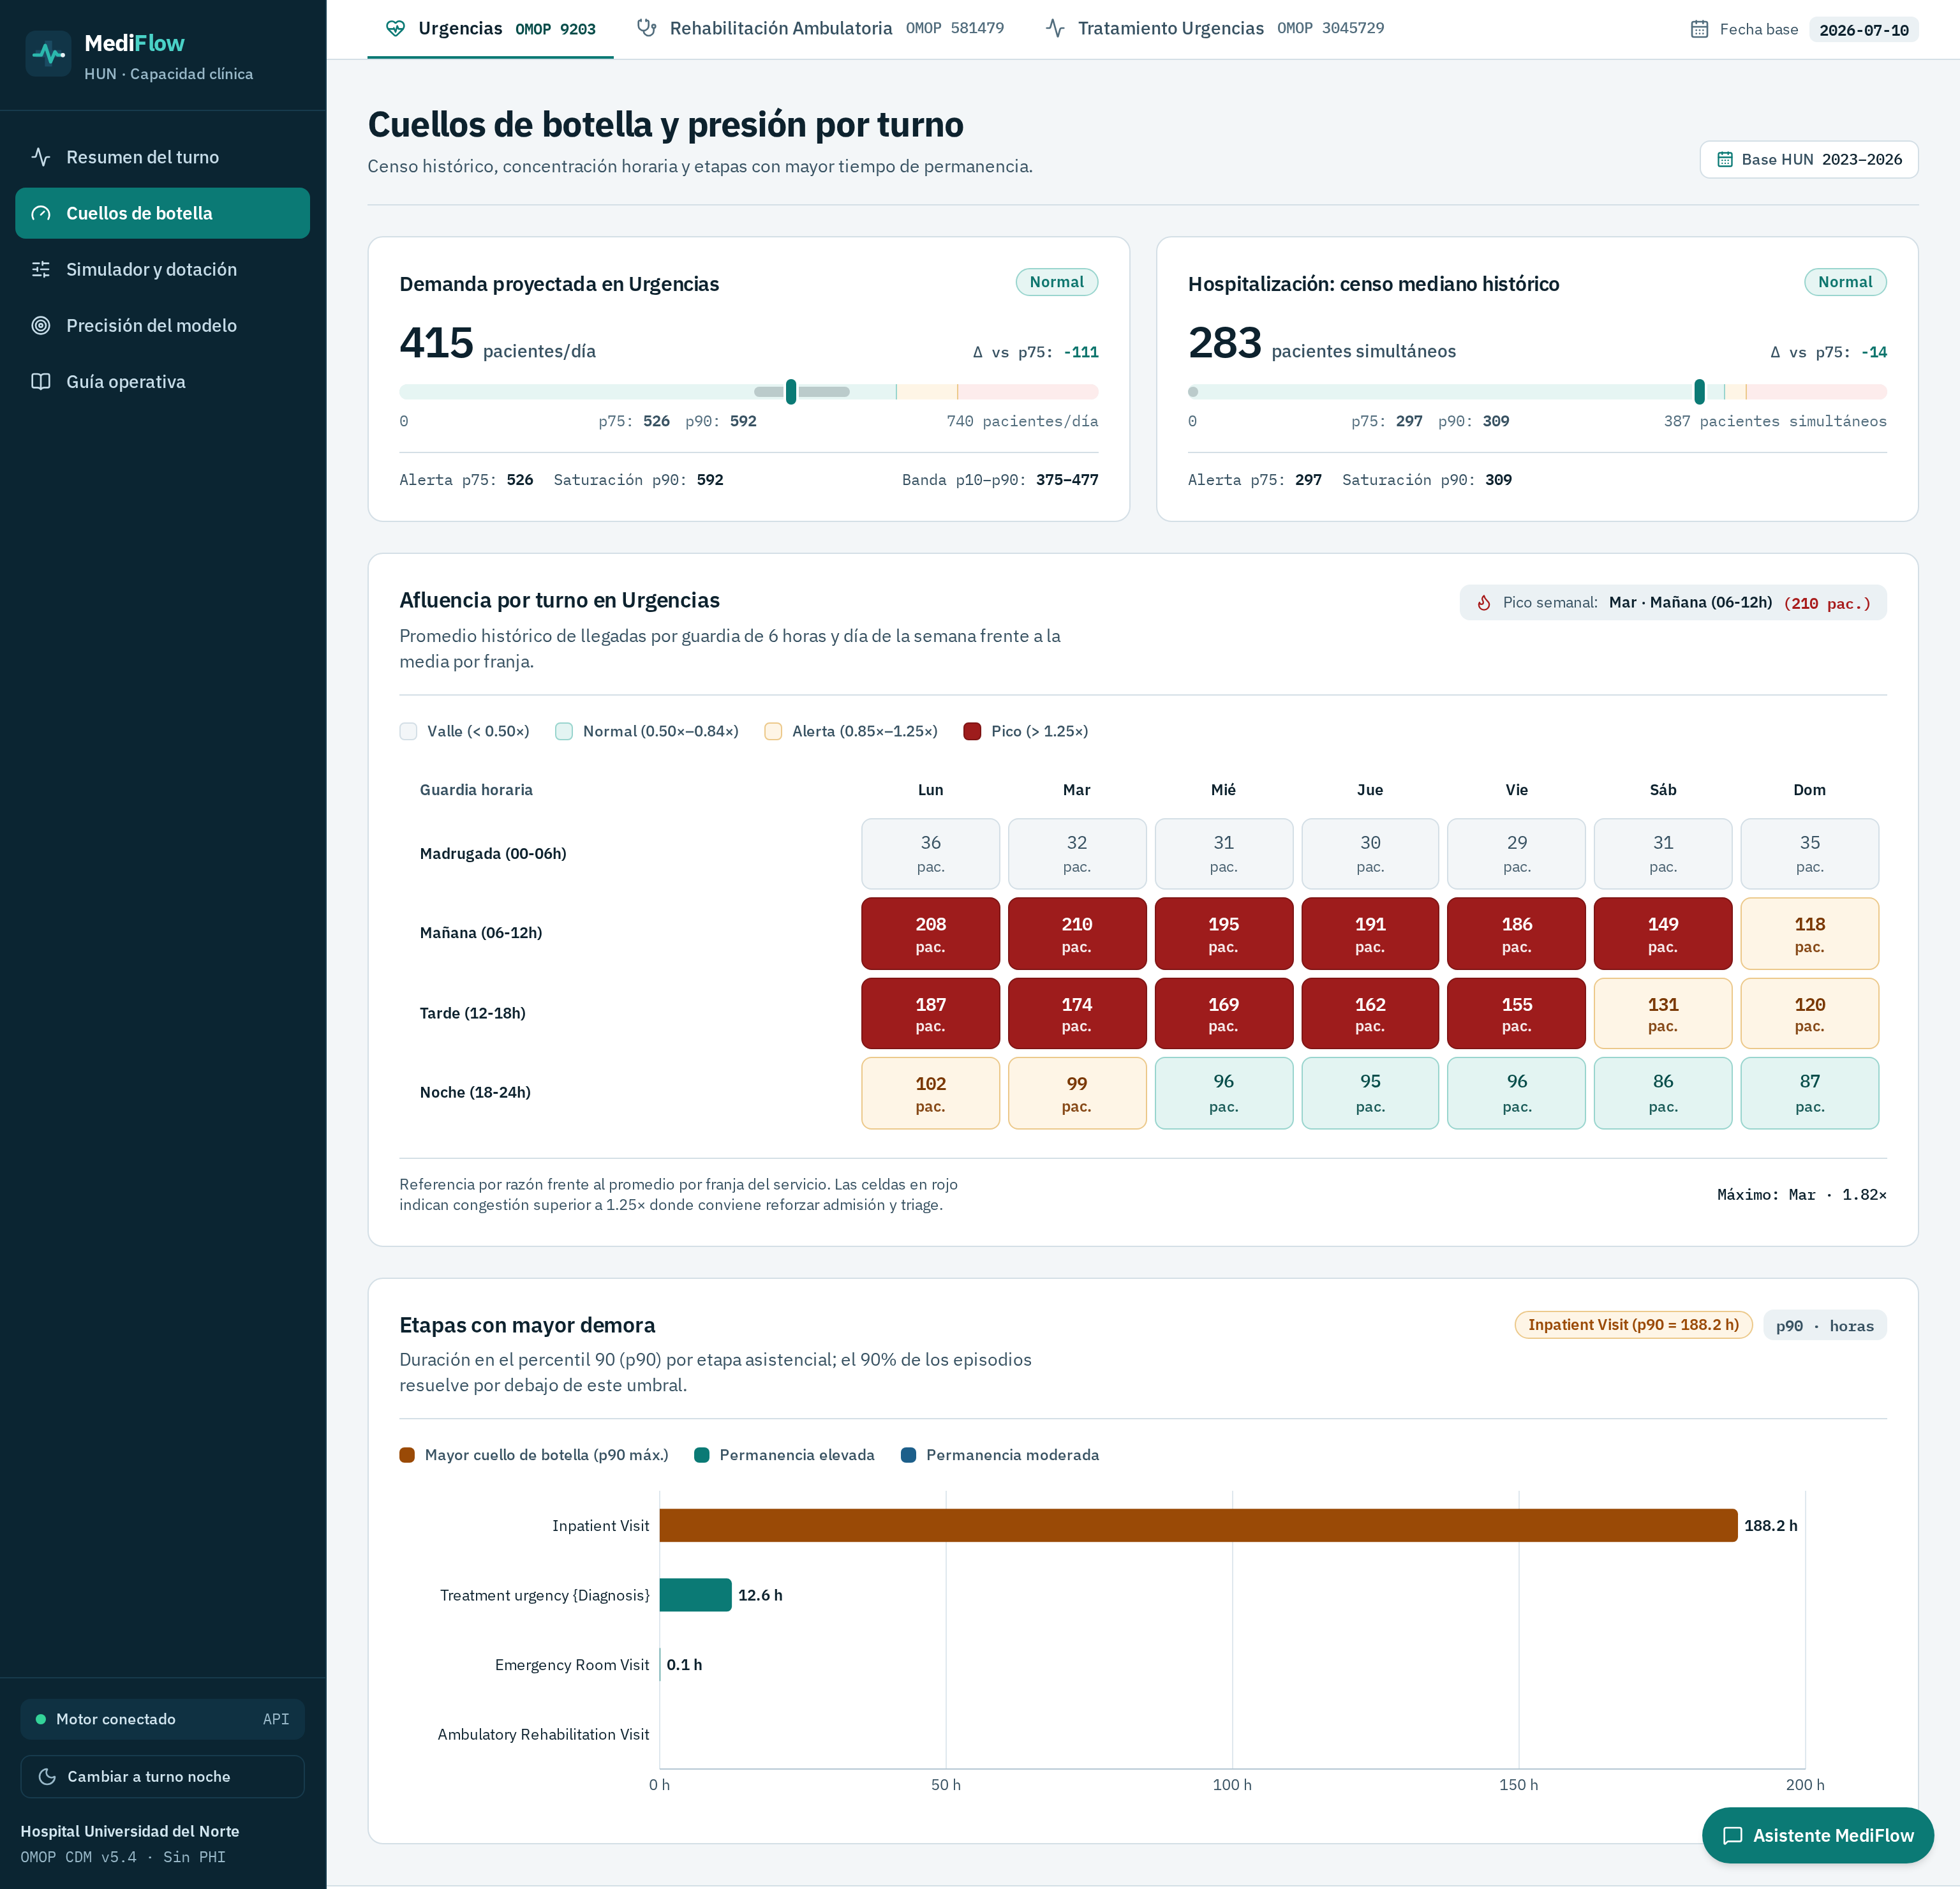
\includegraphics[width=0.92\textwidth]{cuellos_botella.png}
\apanota{Captura archivada del frontend (\texttt{docs/img/app/cuellos\_botella.png}). Muestra indicadores históricos de censo y duraciones por etapa provenientes de agregados del artefacto empaquetado; no representa una ejecución en vivo ni camas físicas habilitadas.}
\end{figure}

\begin{figure}[htbp]
\caption{Vista archivada de precisión histórica en Urgencias con el asistente abierto}
\label{fig:app_precision}
\centering
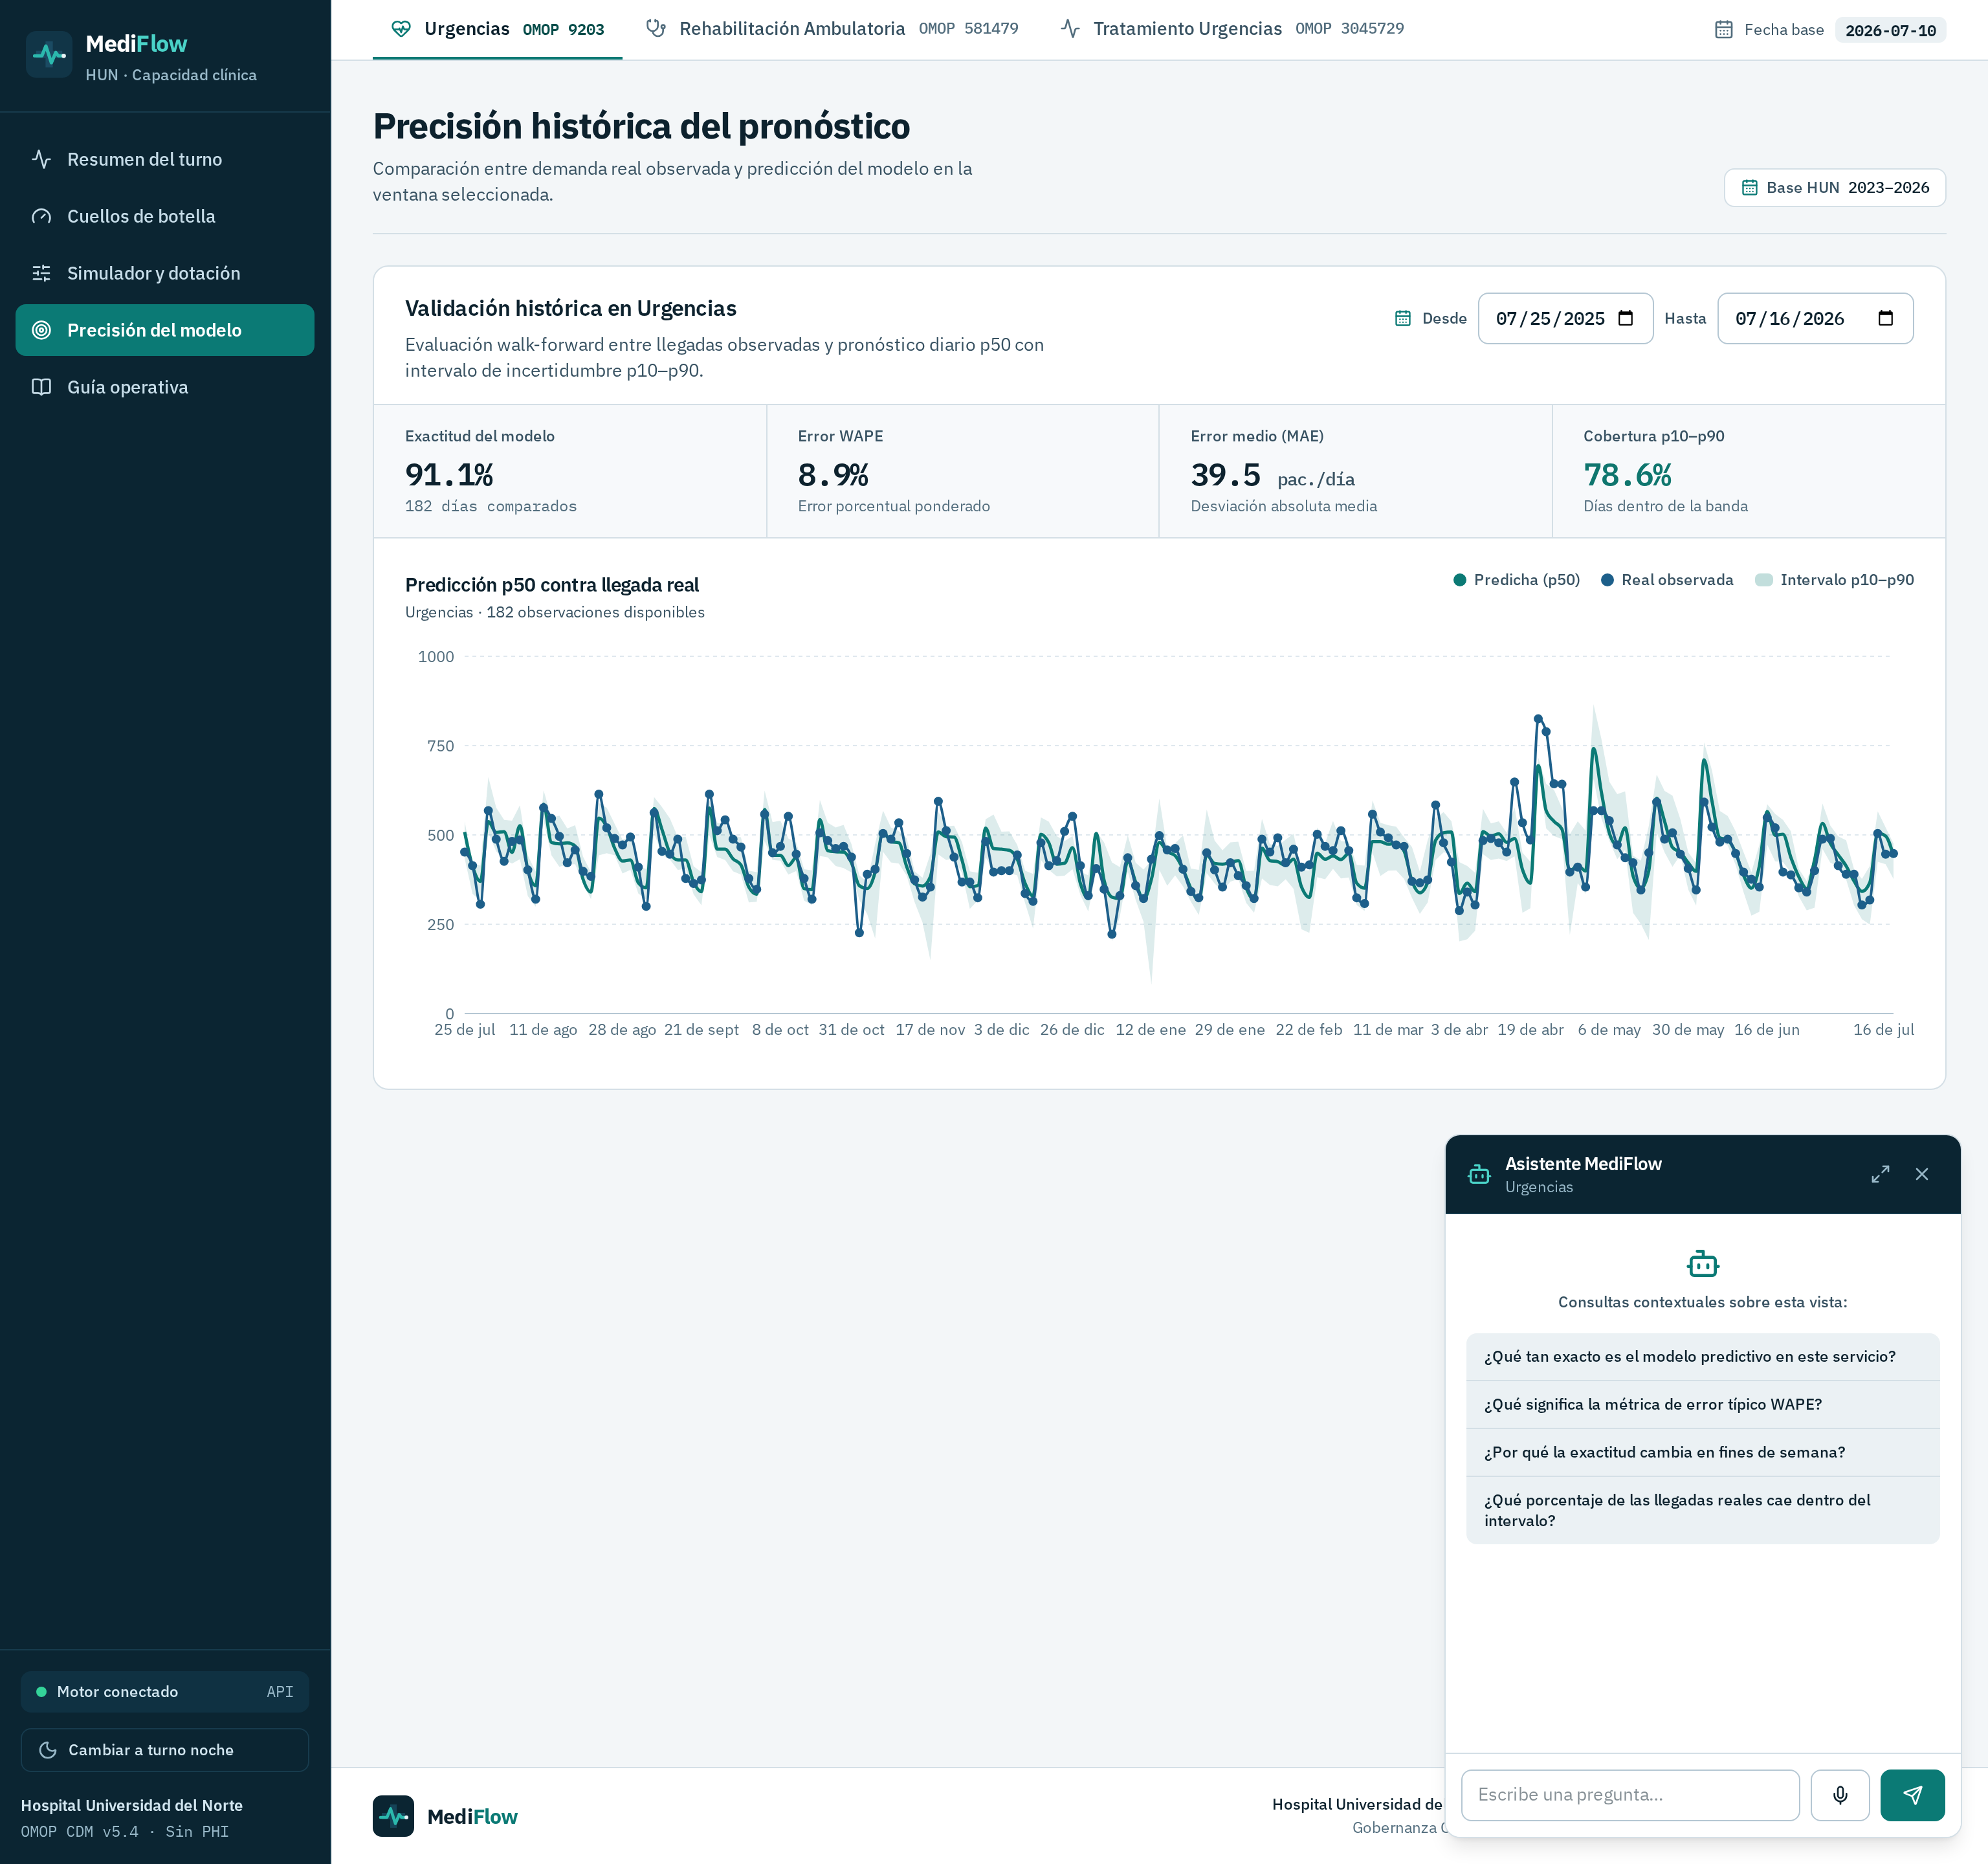
\includegraphics[width=0.92\textwidth]{precision_asistente.png}
\apanota{Captura archivada del frontend (\texttt{docs/img/app/precision\_asistente.png}). Los valores exhibidos (exactitud 91,1\,\%, WAPE 8,9\,\%, cobertura 78,6\,\% en 182 días) corresponden al modelo cuantílico del bundle \texttt{v2.0} y no al experimento puntual Poisson (WAPE 8,4\,\%).}
\end{figure}

\begin{figure}[htbp]
\caption{Captura compuesta archivada del simulador de optimización y escenarios}
\label{fig:app_simulador}
\centering
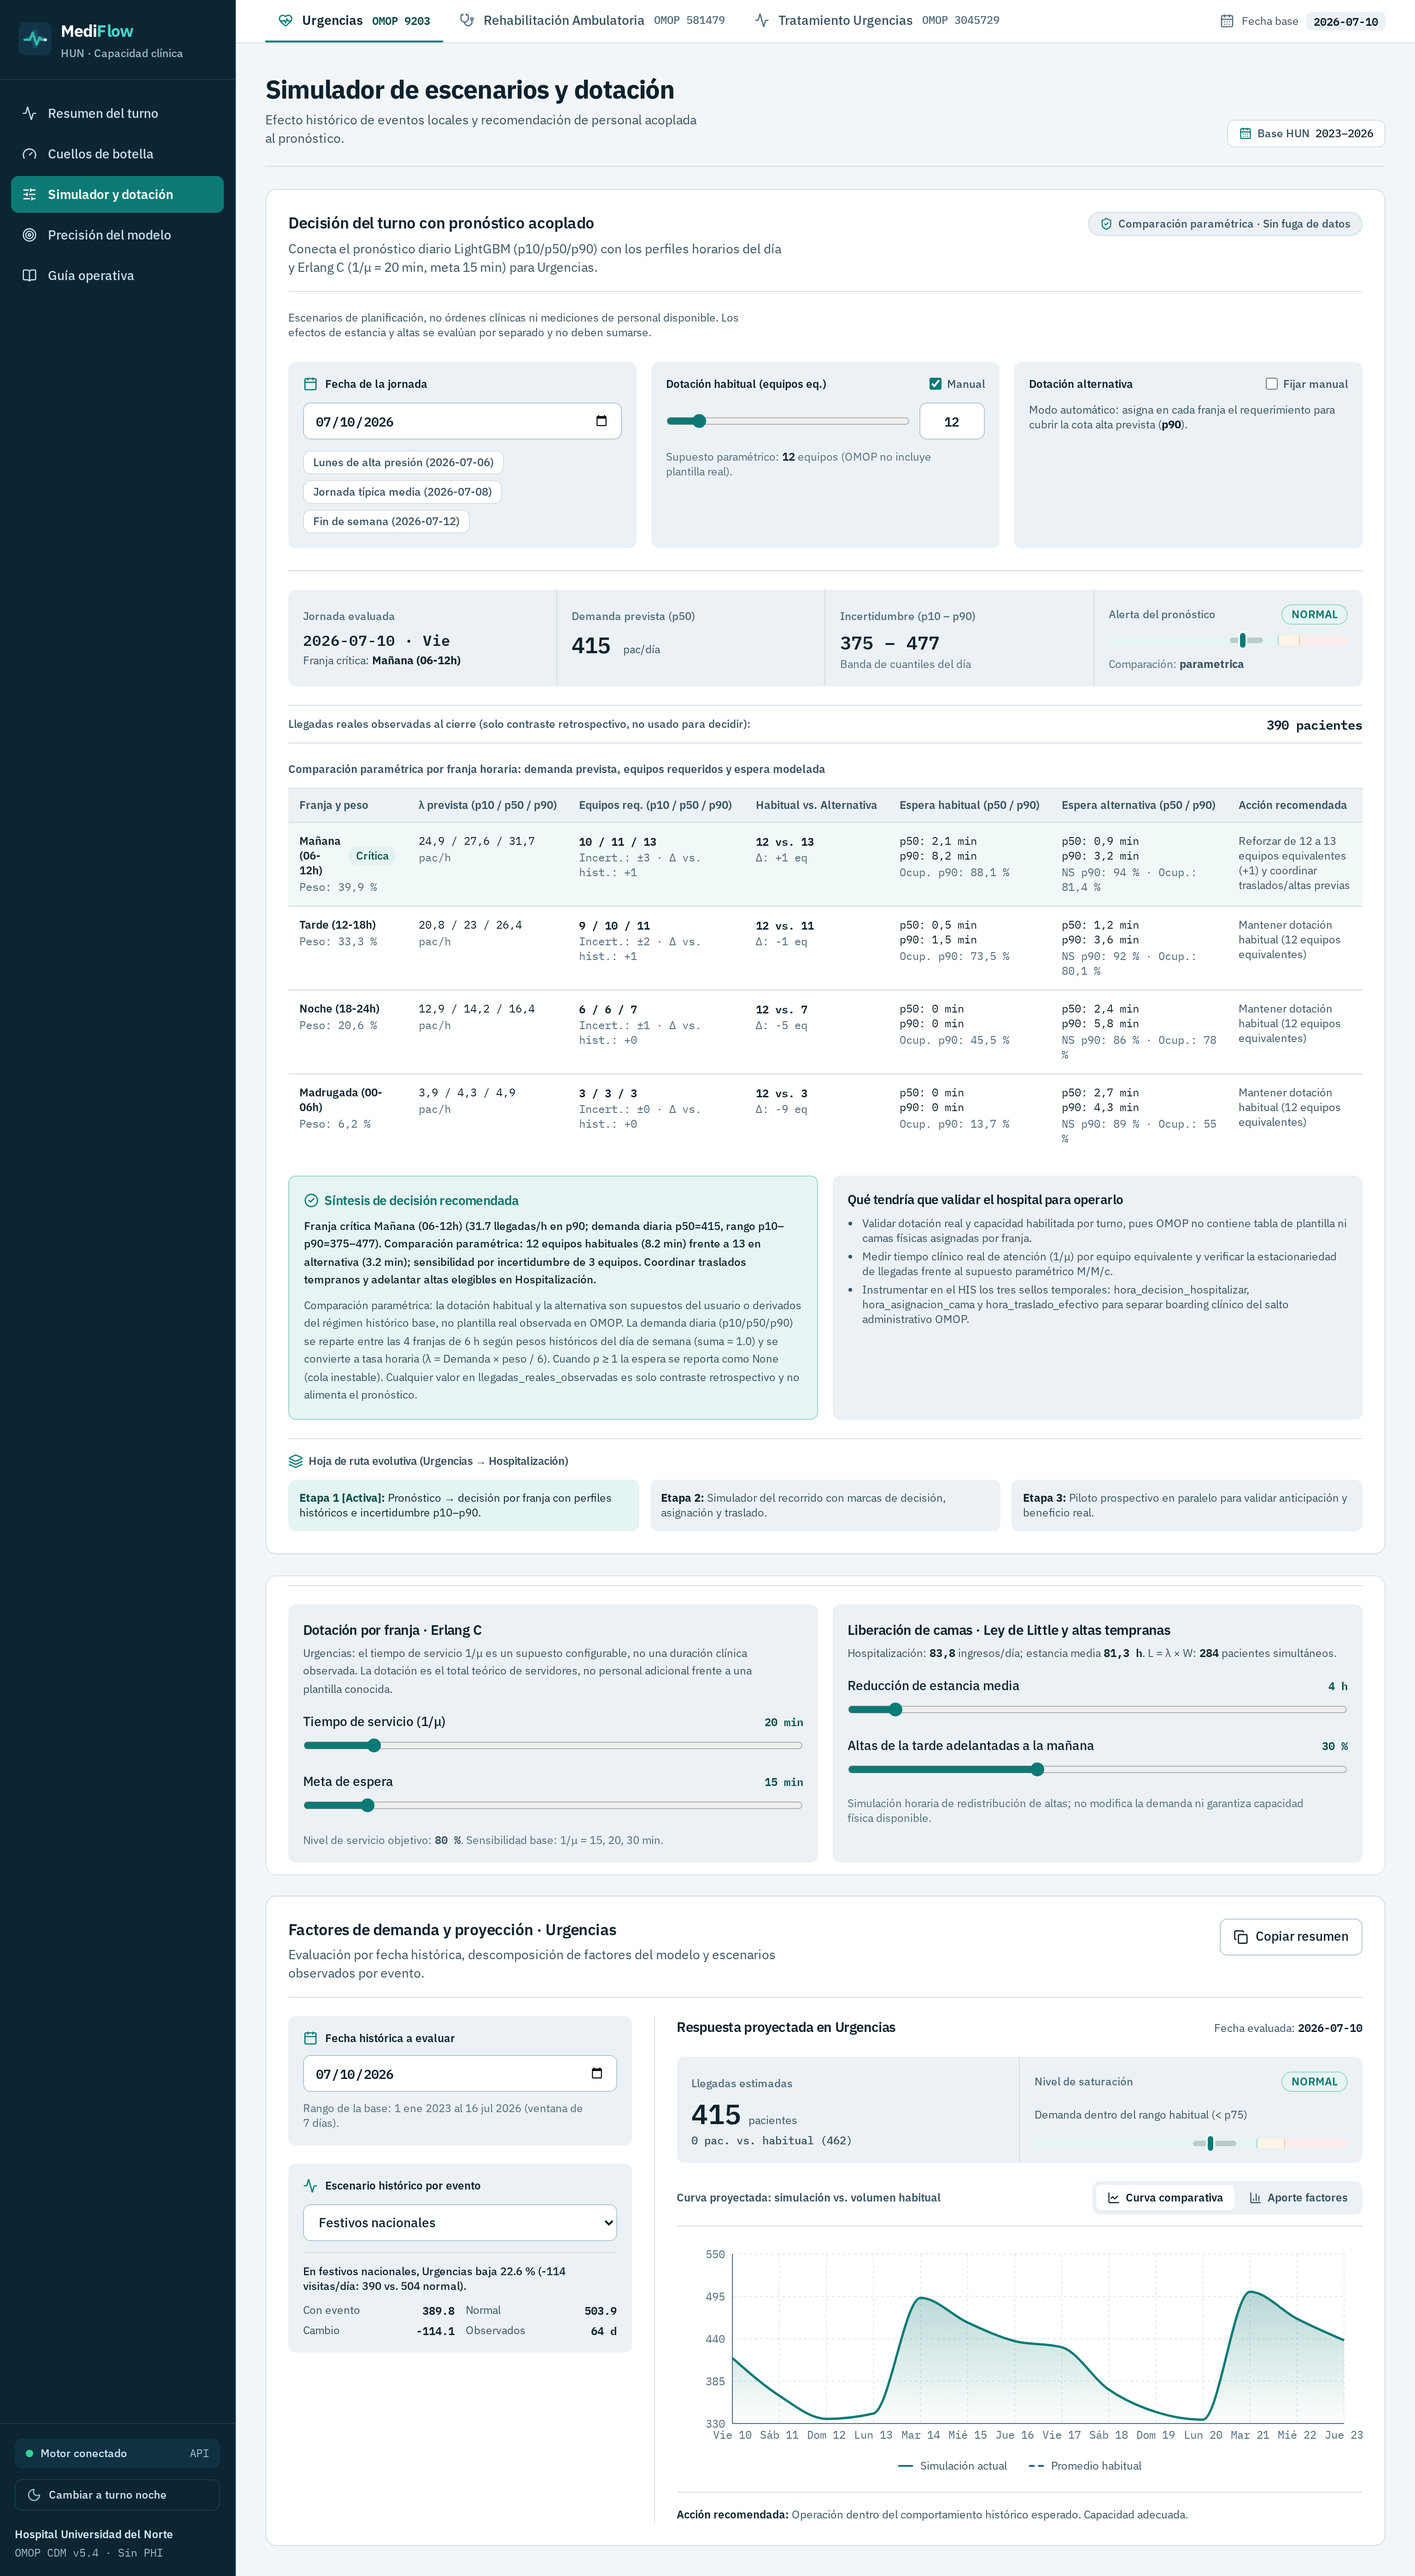
\includegraphics[width=0.92\textwidth,height=0.72\textheight,keepaspectratio]{simulador_optimizacion.png}
\apanota{Captura compuesta archivada (\texttt{docs/img/app/simulador\_optimizacion.png}) que reúne tres secciones verticales de la misma vista. Conserva rótulos anteriores («Etapa 1 [Activa]», «Sin fuga de datos» y referencia híbrida de 284 pacientes en Ley de Little); el código vigente del panel informa explícitamente la ausencia de perfiles por corte en el bundle \texttt{v2.0}.}
\end{figure}

\begin{figure}[htbp]
\caption{Vista archivada del tablero operativo de pronóstico de demanda}
\label{fig:app_dashboard}
\centering
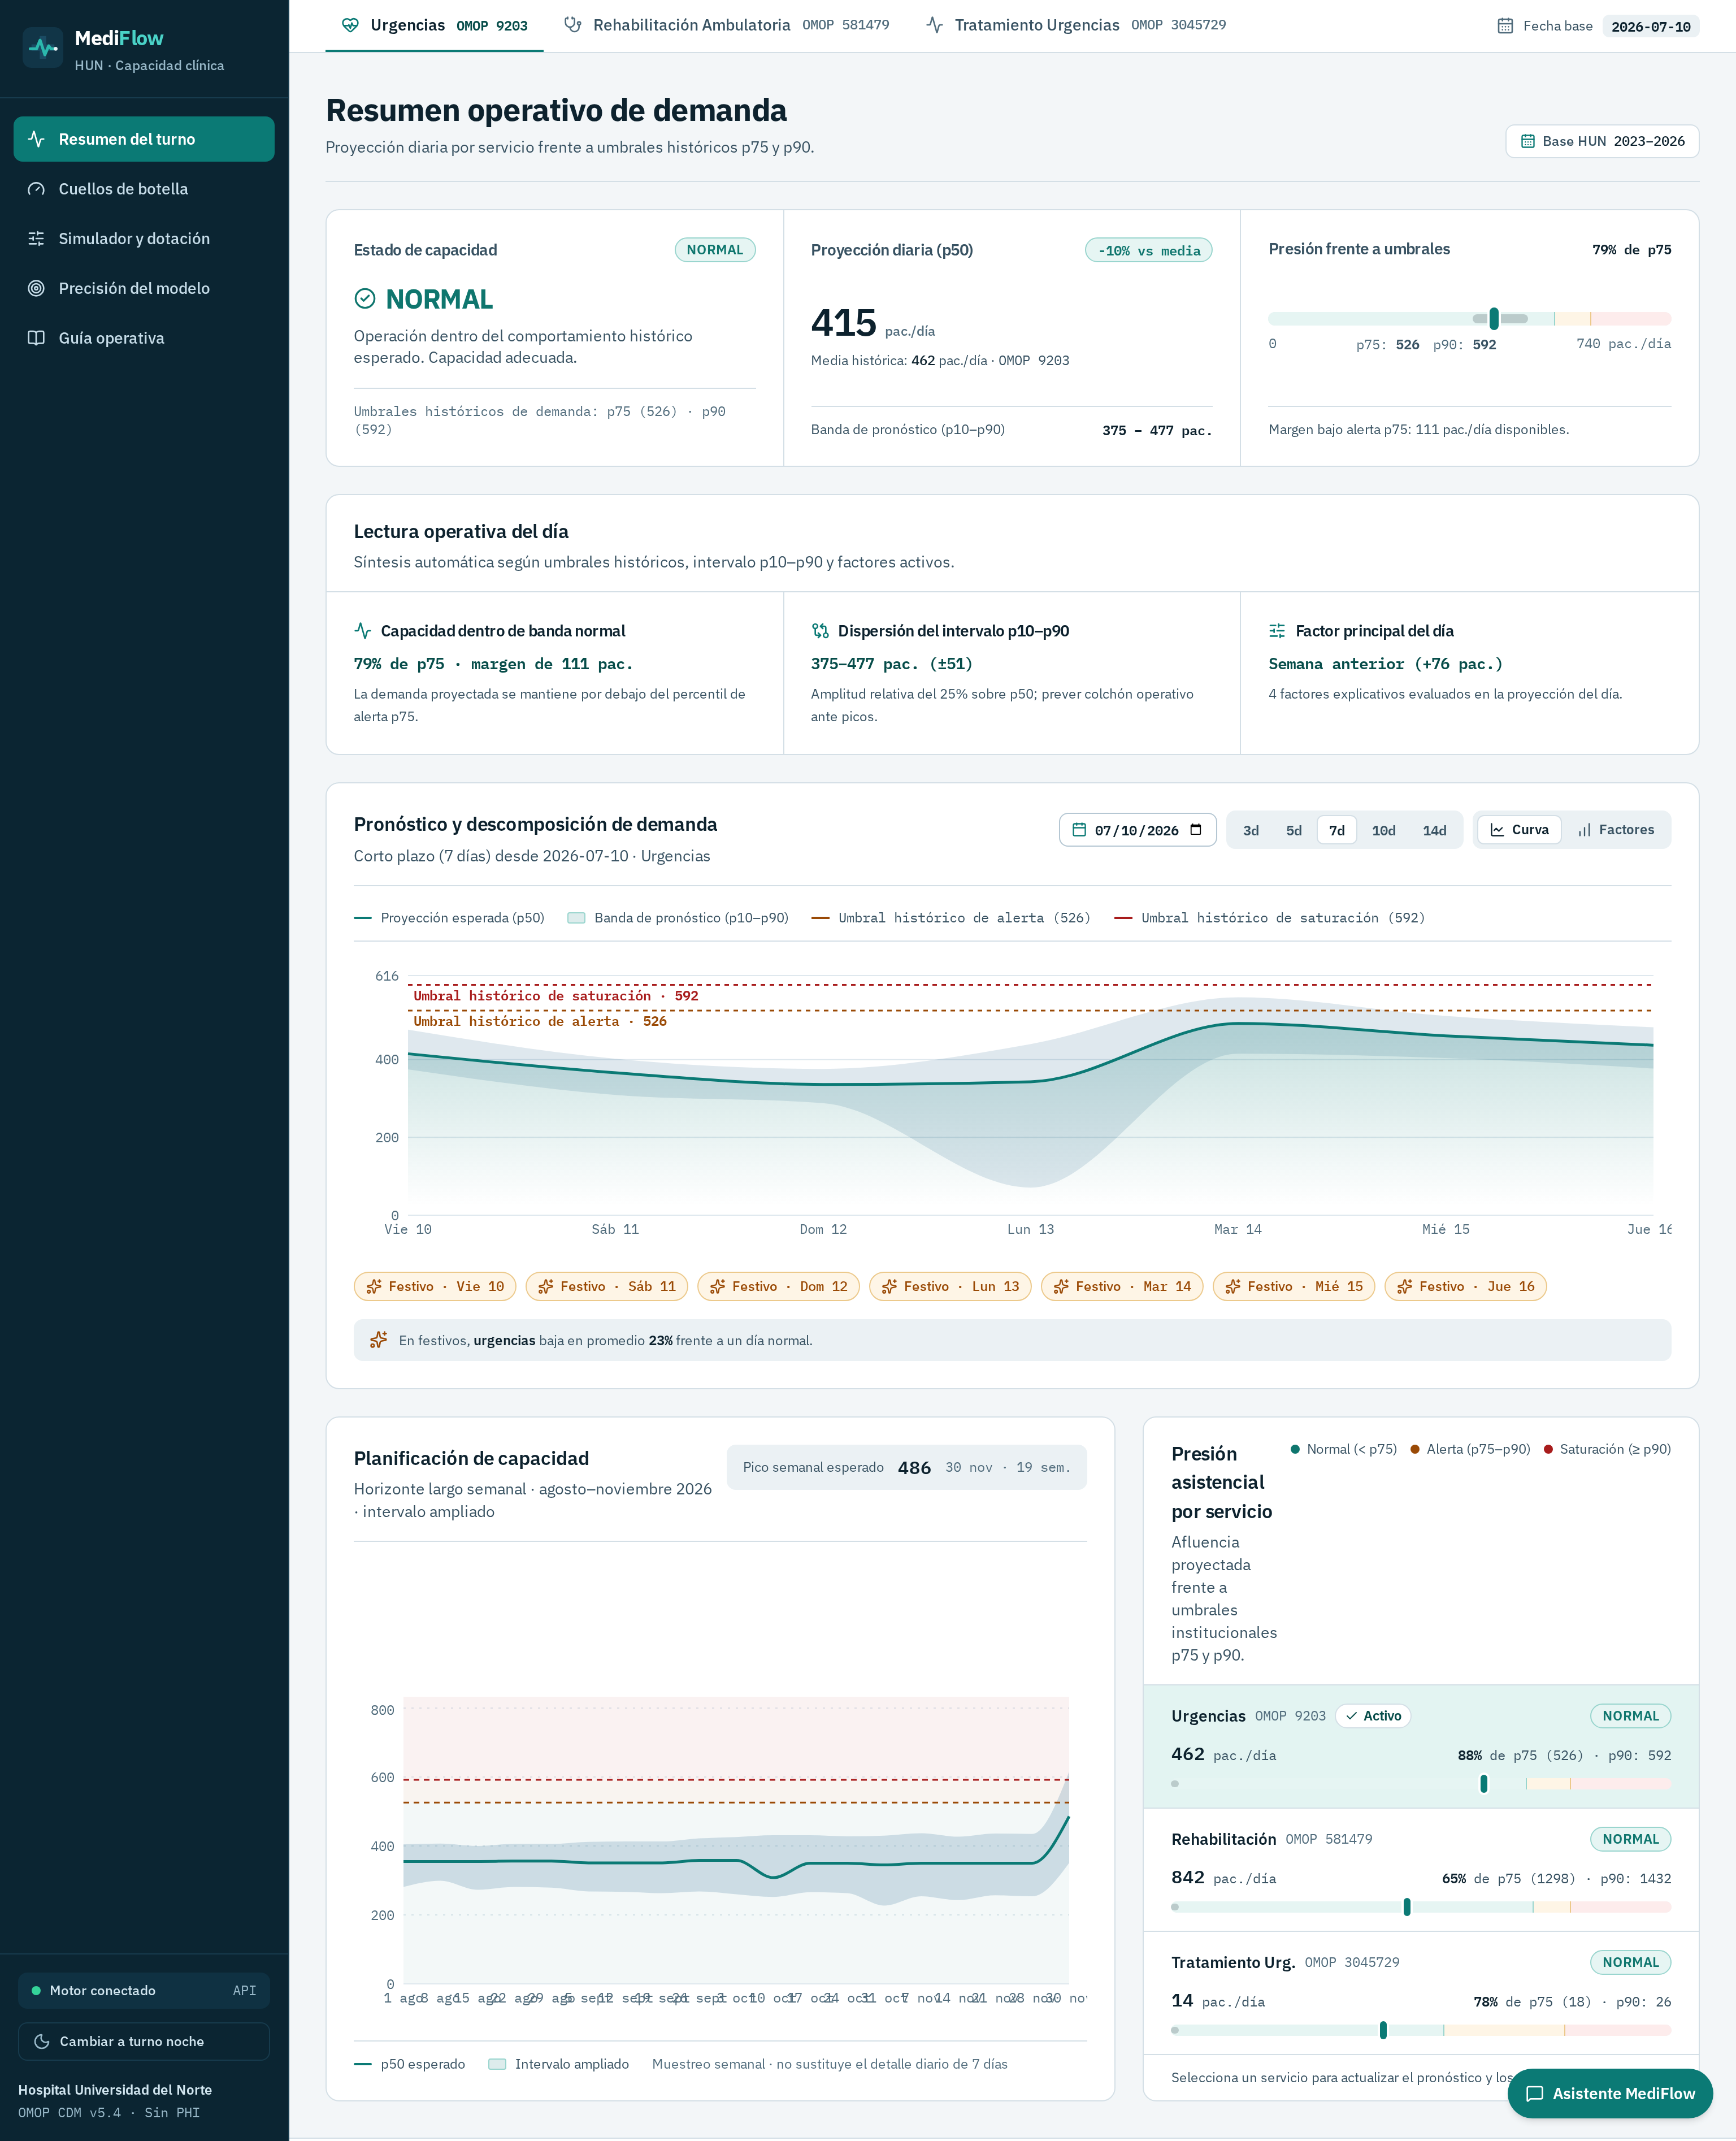
\includegraphics[width=0.92\textwidth,height=0.72\textheight,keepaspectratio]{dashboard_pronostico.png}
\apanota{Captura archivada del frontend (\texttt{docs/img/app/dashboard\_pronostico.png}). Advertencia de integridad visual: la imagen exhibe etiquetas de «Festivo» repetidas sobre los siete días del 10 al 16 de julio de 2026 y superposición de rótulos en el eje temporal del gráfico de largo plazo; debe interpretarse únicamente como ilustración general de diseño y nunca como fuente numérica de calendario ni de proyección.}
\end{figure}
